% !Mode:: "TeX:UTF-8"
%!TEX program  = xelatex
\documentclass[12pt,a4paper]{ctexart}

\usepackage{algorithm2e}
\usepackage{url}
\usepackage{graphicx}
\usepackage{float}
\usepackage{threeparttable}
\usepackage{amsmath}
\usepackage{mathptmx}
\usepackage{amsmath}
\usepackage{amsfonts}
\usepackage{chemformula}
\usepackage{cite}
\usepackage[T1]{fontenc}

\setlength{\parskip}{0.5em}
\title{数字显示温度计大作业}
\author{\textup{李卓壕\quad 曾宸东}}
\begin{document}

\begin{titlepage}
  \newcommand{\HRule}{\rule{\linewidth}{0.5mm}}
  
\includegraphics[width=12cm]{title/logo.png}\\[1cm]
  \center

  \textsl{\Large \textbf{上海交通大学} }\\[0.5cm]
  \textsl{\large \textbf{电子信息与电气工程学院}}\\[0.5cm]
  \makeatletter
  \HRule \\[0.4cm]
  { \huge \bfseries \@title}\\[0.4cm]
  \HRule \\[1.5cm]
  \begin{minipage}{0.4\textwidth}
    \begin{flushleft} \large
      \emph{Author:}\\
      \@author
    \end{flushleft}
  \end{minipage}
  ~
  \begin{minipage}{0.4\textwidth}
    \begin{flushright} \large
      \emph{Superviser:} \\
      \textup{申赞伟}
    \end{flushright}
  \end{minipage}\\[3cm]
  \makeatother

  {\large \emph{EST2503 \quad 电子技术实验}}\\[0.5cm]
  {\large \today}\\[2cm]
  \vfill
\end{titlepage}
\tableofcontents
\section{实验目的}
\subsection{了解PN结温度特性以及通过晶体管构造PN结的方法}
\subsection{学习电压——频率(VF)变换电路的原理}
\subsection{学习精密仪表放大电路的原理及使用}
\subsection{学习如何实现模拟信号到数字信号的转换}
\subsection{学习并掌握Verilog语言的使用}
\subsection{学习利用FPGA设计频率计}


\section{实验内容及原理}

\subsection{模电部分}

\subsubsection{温度传感器}
温度传感器有多种,本实验采用半导体的PN 结作为温度传感器,在一定范围内
PN节的导通压降$U_{on}$就下降2mV。实验中可通过将三极管的BC管脚短路来构造三极管
其中BC为P极,发射结E为N极。具体如下图(1)所示。
\begin{figure}[H]
  \centering
  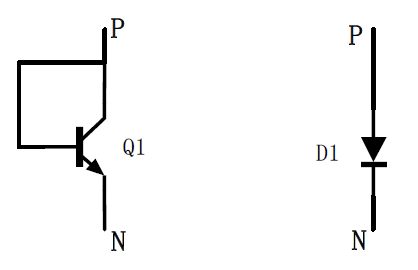
\includegraphics[width=5cm]{pic/2.1.1.png}
  \caption{PN结的实现}
\end{figure}
由于$U_{on}$为PN结的导通电压,因此需要保证PN结处于导
通状态。我们通过设计恒流源来确保PN结的导
通,采用电压——电流转换电路来实现精密恒流源。恒流源的电路图原理
图如图(2)所示。当$R_1=R_2=R_3=R_4=R$时,输出电流与输入
电压满足关系:
\begin{equation}
  i_0=\tfrac{u_I}{R_0}
\end{equation}
\qquad 通过设计参数使得输出电流量级为1-2mA 左右。恒流源电路设计完成后,将输出电阻$R_L$换为晶体管构
成的PN结,即可将其导通电压$U_{on}$稳定输出。为了更好地保护PN结,需要将PN结与一个定值电阻串联
后整体作为$R_L$,在这个状态下输出$U_{on}$。
\begin{figure}[H]
  \centering
  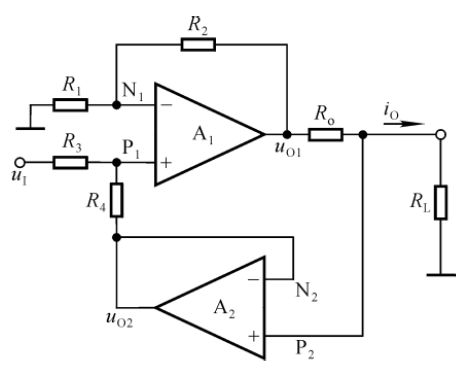
\includegraphics[width=7cm]{pic/2.1.2.png}
  \caption{精密恒流源电路}
\end{figure}

\subsubsection{电压基准源}
\quad PN结电压信号的变化是一个微小量,因此我们用差分放大的思想将其放大。如果将PN结的导通电压
作为放大器一端的输入,则另一个输入应该为与$U_{on}$大小相近的恒定量,该恒定量与$U_{on}$做差所得到的微
小量则是待放大的电压信号。因此我们需要得到一个与$U_{on}$相近的恒定量。我们采用TL431 精密电压参
考源作为电压基准源,来实现恒压输出。


TL431 集成电压基准电路的内部结构、典型接线及引脚分布如图(3)所示。将该电路与可变电阻相连接,
通过改变可变电阻阻值则可得到希望的恒压输出量。

\begin{figure}[H]
  \centering
  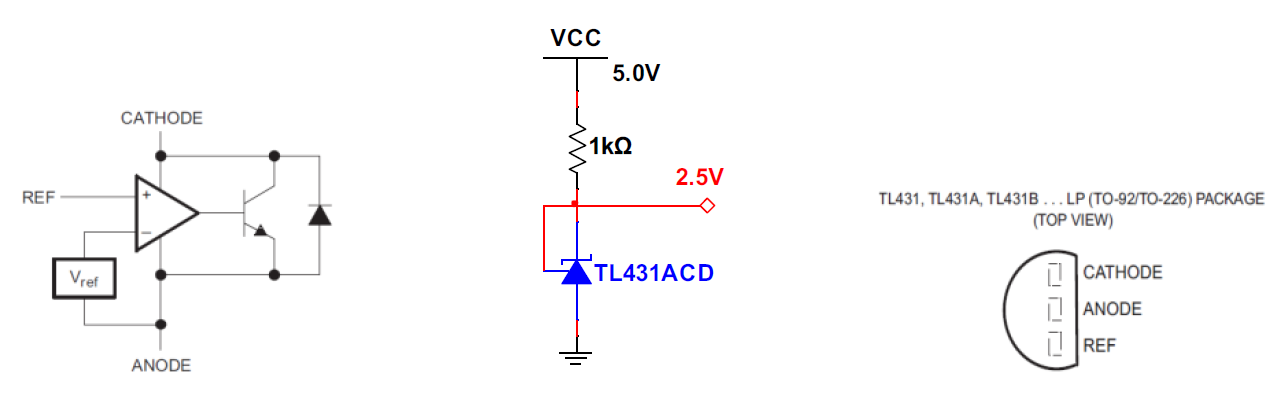
\includegraphics[width=12cm]{pic/2.1.3.png}
  \caption{TL431 集成电压基准电路的内部结构、典型接线及引脚分布}
\end{figure}

\subsubsection{电压差分放大电路}
差分放大电路用于放大电压基准源与PN结导通压降之差,我们使
用精密(仪表)放大电路进行实现。电路原理图如
图(4)所示。输出电压与两端的输入满足表达式:

\begin{equation}
  u_0=-\tfrac{R_f}{R}(1+\tfrac{2R_1}{R_2})(u_{I1}-u_{I2})
\end{equation}

放大的范围需要满足PN 结电压在变化为$2mV*100=200mV$
的情况下,仪表放大器的输出为5V左右。其中
增益的调整由$R_2$实现,所以实际电路$R_2$采用可变电阻。考虑到输出电压的表达式含有
负号,我们将导通压降$U_{on}$作为$u_{I1}$端的输入,将基准源作为$u_{I2}$端的输入。
当温度升高时,$U_{on}$不断减小,使得$u_{I1}-u_{I2}<0$,以保证输出电压$u_o>0$。

\begin{figure}[H]
  \centering
  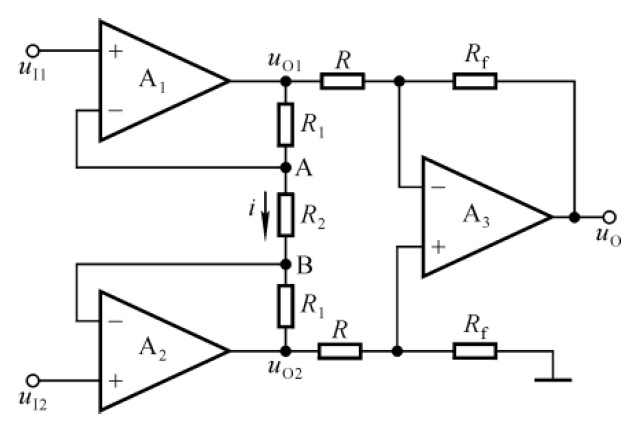
\includegraphics[width=7cm]{pic/2.1.4.png}
  \caption{精密(仪表)放大电路}
\end{figure}

\subsubsection{F-V伏频转换电路}
电压进行放大后,我们需要将电压信号进一步转换为频率信号,频率信号可通过FPGA进行处理。我们希
望的输出是当温度由0℃至100℃变化时,输出信号的频率由0Hz 至10KHz 线性变化,也就是将输入信号
$u_I$的0~5V映射至频率区间0~10kHz。其中,双向稳压管由两个单向稳压管反向串联实现。使用如下的F-V
幅频转换电路,电路见图(5)所示。经过电容的充放电作用,周期T与$u_I$及电路参数的关系为:
\begin{equation}
  T=R_1C*\tfrac{U_{REF}}{u_I}
\end{equation}

\begin{figure}[H]
  \centering
  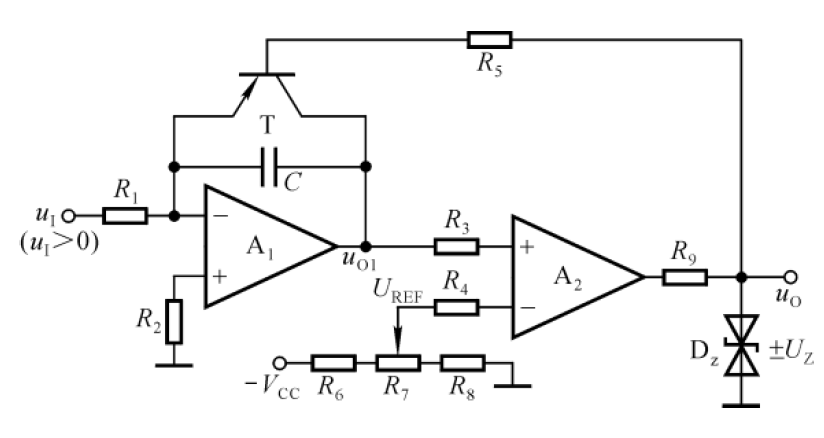
\includegraphics[width=9cm]{pic/2.1.5.png}
  \caption{电压-频率(V-F)变换电路}
\end{figure}

\subsubsection{3.3V电平转换电路}
最后,输入FPGA的信号大小需要进行限制,防止烧坏FPGA。我们将输出的$\pm U_Z$转换成为0-3.3V 电
平,以匹配数字电路部分的FPGA
开发板的输入电平。电路实现如图(6)所示。
\begin{figure}[H]
  \centering
  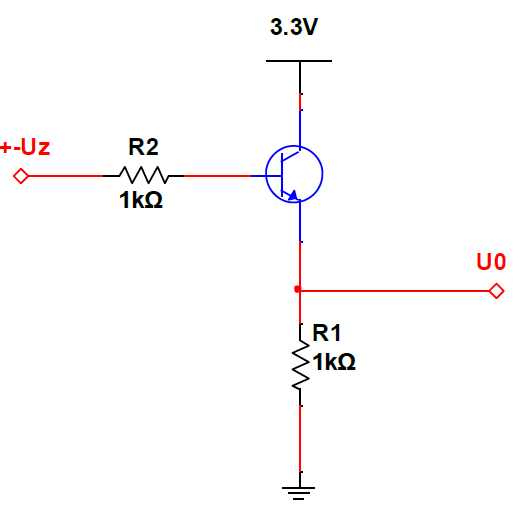
\includegraphics[width=7cm]{pic/2.1.6.png}
  \caption{3.3V 电平转换电路}
\end{figure}

\subsubsection{模拟部分总结}
模拟部分实现将温度信号进行调理放大,变换为频率信号,最终以3.3V 的频率信号(0-10kHz)输
出,频率的大小与温度成正比。

\end{document}

